\documentclass{article}
\usepackage{amsmath}
\usepackage{amssymb}
\usepackage{fancyhdr}
\usepackage[papersize={8.5in,11in}, margin={1in}]{geometry}
\setlength{\headheight}{40pt}
\fancyhead[L]{CS 5800 \\ Lecturer: James Kim \\ Problem Set 4}
\fancyhead[R]{Student: Rongfei Jin}
\renewcommand\headrulewidth{0.4pt}
\pagestyle{fancy}

\usepackage{graphicx}
\graphicspath{{./images/}}

\setlength{\parindent}{0pt}

\title{Problem Set 4 Solution}
\author{Rongfei Jin}
\date{\today}
\begin{document}

\section*{Question 1}
\subsection*{Solution to (a)}
\begin{figure}[h]
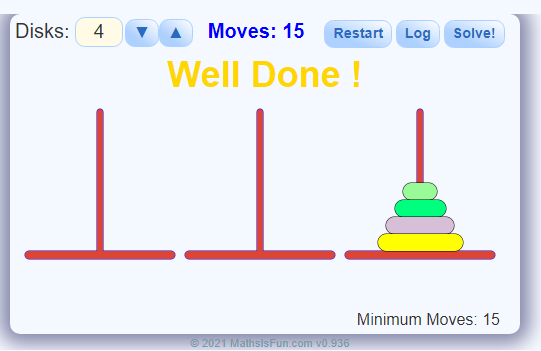
\includegraphics[scale=0.4]{1-1.png}
\end{figure}

\subsection*{Solution to (b)}
    
Denote Disk 1-4 (ascending in size) as D1, D2, D3, D4. and Tower 1-3 as T1, T2, T3. And denote the set of disk on one tower as D12 (disk 1 and 2), D123 (disk 1, 2, 3), etc.

\vspace{3mm}

To win the game, we need move all disk from t1 to t3, and since the placement of disks are strictly in desceding order, the largest disk d4 should be the first disk to move to t3. And the second largest follows, then the third largest, and the smallest disk d1 should be the last disk to move to t3.

Therefore, the total number of steps to move all 4 disks is:
\[T(4) = T(\text{D4 T1 to T3}) + T(\text{D3 T1 to T3}) + T(\text{D2 T1 to T3}) + T(\text{D1 T1 to T3})\]

However, it is hard to track the number of steps for each disk to move to t3 directly. Therefore, we can break down the problem into smaller subproblems by considering the the movement of D123 from T1 to T3 as a whole, this gives us the following equation:

\[T(4) = T(\text{D4 T1 to T3}) + T(\text{D123 T1 to T3}) \]

And for D4 to move to T3, we also need to move D1-3 to T2 first, and then move D4 to T3, and then move D1-3 to T3. Therefore, the total number of steps for D4 to move to T3 is:


\[T(4) = 1 + T(\text{D123 T1 to T2}) + T(\text{D123 to T3}) \]

Considering T123 from T1 to T2 and T1 to T3, because there's no T4 restrict the movement, the number of steps for T123 to move to T2 and T3 are the same. Therefore, we have:

\begin{align*}
T(4) &= 1 + T(\text{D123 T1 to T3}) + T(\text{D123 to T3}) \\
&= 1+ 2T(3) \\
&= 15
\end{align*}

And because \(T(3)\) is given as the minimum number of steps to move 3 disks from T1 to T3, we have \(T(3) = 7\). Therefore, the minimum number of steps to move 4 disks from T1 to T3 is 15.


\newpage

\subsection*{Solution to (c)}

To find the recursive relation, we should first find the recursive relation for \(T(3)\).
It is easy to see that to move D3 to T3, we need to move D12 to T2 first, then move D3 to T3, and then move D12 to T3. 
This gives us the following relation:

\[T(3) = 1+2T(2)\]

And the recursive relation for \(T(2)\) is almost trivial, we simply move D1 to T2, then move D2 to T3, and then move D1 to T3. Therefore, we have:

\[T(2) = 1+2T(1)\]

Based on the solution to (b), we can derive the following relation:

\begin{align*}
T(4) &= 1 + 2T(3) \\
T(3) &= 1 + 2T(2) \\
T(2) &= 1 + 2T(1) \\
T(1) &= 1
\end{align*}

Then consider we have k where \(k>4 \, k\in \mathbb{Z^+}\) disk. In order to move Dk to T3, we need to move D1 to Dk to T2 first, then move Dk to T3, and then move D1 to Dk to T3. This is the minimal move for every level of k, since you must have T3 cleared as well as every disk above Dk removed before move Dk to T3, which results in a D1 to DK on T2. In addition, move D1 to Dk to D2 and to D3 are 2 same sets of movements since there's no Dk to restrict the movement of D1 to Dk and one can switch the role of T2 and T3. 

Therefore we propose a recurrence relation for \(T(n)\):
\[T(n) = 1 + 2T(n-1)\]

Then we can solve this recurrence relation by substitution method:

\begin{align*}
T(n) &= 1 + 2T(n-1) \\
&= 1 + 2(1 + 2T(n-2))  = 1 + 2 + 4T(n-2) \\
&= 1 + 2 + 4(1 + 2T(n-3)) = 1 + 2 + 4 + 8T(n-3) \\
&= \ldots \\
&= \left( 1 + 2 + 4 + 8 + \ldots + 2^{k-1} \right) + 2^{k} T(n-k) \\
\end{align*}

where \(0 < k < n, k \in \mathbb{Z}\) 

The recursion stops when \(n-k = 1 \Rightarrow k = n-1\). Therefore, the minimal total number of steps to move n disks from T1 to T3 is:

\begin{align*}
    T(n) &= \sum_{i=0}^{n-2} 2^i + 2^{n-1} \cdot  1 \\
    &= \frac{(2^{n-1})-1}{2-1} + 2^{n-1}  && \text{geometric seris sum of } n - 1 \text{ terms} \\
    &= 2^{n-1} - 1 + 2^{n-1}\\
    &= 2^n - 1
\end{align*}

\newpage

\subsection*{Solution to (d)}

Let \(n = \log(m)\). The relation becomes 
\[
T(\log(m)) = 2T(\log(m)-1) + 1 = 2T(\log(\frac{m}{2})) + 1
\]

Define \(S(m) = T(\log(m))\), then we have
\[S(m) = 2S(\frac{m}{2}) + 1\]

This has the form required by master theorem, where \(a = 2, b = 2, f(n) = 1 \text{ and is asymptotic positive}\).

\vspace{3mm}

Check case of 1 master theorem: If \(f(n) = O(n^{\log_b a - \epsilon})\) for some \(\epsilon > 0\), then \(S(m) = \Theta(n^{\log_b a})\).
- This is true because \(f(n) = O(n^{\log_b a - \epsilon})\) for \(\epsilon = 1\), since \(1 = O(n^{1-1})\).

Therefore, the solution is:
\[S(m) = \Theta(m)\]

since \(n = log(m) \rightarrow m=2^{n}\), we have:

\[T(n) = S(2^m) = \Theta(2^n)\]

So from (c) we have \(T(n) = 2^n - 1\), and by the definition of \(\Theta\), we can find \(c_1>0, c_2>0, n_0\ge 0 \) such that:

\[c_1 \cdot 2^n \leq 2^n - 1 \leq c_2 \cdot 2^n \text{ for all } n \geq n_0\]

let's choose \(c_1 = 0.5, c_2 = 1, n_0 = 1\), then we have:

\[2^{n-1} \leq 2^n - 1 \leq 2^n \text{ for all } n \geq 1\]

The upper bound is trivial to verify, and the lower bound  is also true since:
\begin{align*}
    c_0\cdot 2^{n} &\leq 2^n - 1 \\
    1 &\leq 2^{n} (1 - c_0) \\
    1 - c_0 &\ge \frac{1}{2^n} \\
    c_0 &\leq 1 - \frac{1}{2^n}
\end{align*}

sub in \(n=1\), we have \(c_0 \leq 0.5\), therefore, the \(c_0 = 0.5\) works

\newpage

\section*{Question 2}
\subsection*{Solution to (a)}

\begin{align*}
A &=[3, 1, 5, 7, 6, 2, 4] \\
&= [3, 1, 2, 7, 6, 5, 4] && \text{swap 2 and 5} \\
&= [3, 1, 2, 4, 6, 5, 7] && \text{swap 4 and 7} \\
\end{align*}
\(q = 4 \)

Partition(\(p = 1, r = 4-1 = 3\))
\begin{align*}
    A_1 &= [3, 1, 2] && \text{pivot is 2} \\
    &= [1, 3, 2] && \text{swap 1 and 3} \\
    &= [1, 2, 3] && \text{swap 2 and 3} \\
\end{align*}
\(q=2\) Cannot partition further with \(partition(1, 1)\) and \(partition(3,3)\)

Partition(\(p = 5, r = 7\))
\begin{align*}
    A_2 &= [6, 5, 7] && \text{pivot is 7} \\
    &= [6, 5, 7] && \text{no swap} \\
\end{align*}
\(q=7\) Cannot partition further with \(partition(8,7)\)

Partition(\(p = 5, r = 6\))
\begin{align*}
    A_3 &= [6, 5] && \text{pivot is 5} \\
    &= [5, 6] && \text{swap 5, 6} \\
\end{align*}
\(q=5\) Cannot partition further with \(partition(5,4)\) or \(partition(6,6)\)

Since the sort is done in each partition, the final sorted array is:
\[A = [1, 2, 3, 4, 5, 6, 7]\]

\newpage

\subsection*{Solution to (b)}

This is a sorted array, so the partition will always be on the left side of the pivot. Therefore, the number of comparisons is the sum of the first n-1 integers

\begin{align*}
A_0 &=[1, 2, 3, 4, 5, 6, 7] && \text{ number of comparison is 6} \\
A_1 &=[1, 2, 3, 4, 5, 6] && \text{ number of comparison is 5} \\
A_2 &=[1, 2, 3, 4, 5] && \text{ number of comparison is 4} \\
A_3 &=[1, 2, 3, 4] && \text{ number of comparison is 3} \\
A_4 &=[1, 2, 3] && \text{ number of comparison is 2} \\
A_5 &=[1, 2] && \text{ number of comparison is 1} \\
\end{align*}

\[
n = 1+2+3+4+5+6 = 21
\]

\newpage
\subsection*{Solution to (c)}

Suppose the partition is based on a value p, where \(0<p<1\), so approximately each time parititon will have \(np\) and \(n(1-p)\) elements. We can then express the number of comparison as:
\[T(n) = T(pn) + T((1-p)n) + n-1\]

And we know that quick sort has the best case \(O(n\log n)\). We then try substituing \(T(n) = n\log n\), since we want to know the best case with least comparison, which gives us:

\begin{align*}
T(n) &= (pn) \log pn + (1-p)n \log (1-p)n + n - 1 \\
\end{align*}

To find which p gives the minimum number of comparison, we can take the derivative of T(n) with respect to p and set it to 0:
\[
\frac{\partial}{\partial p} T(n) = 0
\]

\[
n^2\log p + n^2\log (1-p) = 0
\]

\[p = 0.5\]


Therefore, the best case is to have the partition as close to the middle as possible, which is to have the pivot as the median of the array.

Therefore, given a sorted array, \[[a_1, a_2, a_3, a_4, a_5, a_6, a_7]\] where \(a_i < a_j\) for \(i < j\), the best case is to have the pivot as \(a_4\), which is the median of the array. We will put \(a_4\) as the pivot, then we will have two partitions which we don't know the order,

\[A = [[a', a'', a''], a_4, [a'''', a''''', a'''''']]\]

Similarly, we will put the median of the two partitions as the pivot,

\[A_1 = [[a', a''], a_2], A_2 = [[a''', a'''''], a_6]\]


Since there's only one way to partition a size of 2 array, the order can be arbitrary

And then we can merge the two partitions to get the original array. Here \(a_6, a_4\) are swapped to get the original array
\[A = [a', a'', a_2, a_6, a''', a'''', a_4]\]

This will give us the minimum number of comparisons 10. A permutation run verify that this is the best case.
\newpage
\subsection*{Solution to (d)}

The best case is to have the pivot as the median of the array, which is the middle element of the array. Therefore, the recurrence relation is: \[T(n) = n - 1 + 2T(n/2)\]

This has the form required by master theorem, where \(a = 2, b = 2, f(n) = n \text{ and is asymptotic positive}\).

\vspace{3mm}

Check case of 1 master theorem: If \(f(n) = O(n^{\log_b a - \epsilon})\) for some \(\epsilon > 0\), then \(T(n) = \Theta(n^{\log_b a})\).

This case does not hold because \(f(n) = O(n^{\log_b a - \epsilon})\) for \(\epsilon = 1\), since \(n \ne O(n^{1-1})\). 

\vspace{3mm}

Check case of 2 master theorem: If \(f(n) = \Theta(n^{\log_b a}
log^k(n))\), then \(T(n) = \Theta(n^{\log_b a} \log^{k+1} n) \, k\ge 0\).
This case holds for \(k=0\) because \(f(n) = \Theta(n^{\log_b a})\), since \(n = \Theta(n^{\log_2 2}) = \Theta(n)\).

Therefore, T(n) = \(\Theta(n \log n)\)

\vspace{6mm}

In the worst case, the pivot is the smallest or largest element of the array, which is the first or last element of the array. Therefore, the recurrence relation is: \[T(n) = n - 1 + T(n-1) = n + (n-1) + \ldots + 1 = \sum_{i=1}^{n-1} i\]

This is a arithmetic series, and the sum of the series is \(\frac{n(n-1)}{2}\). Therefore, the worst case is \(T(n) = O(n^2)\)

\newpage

\section*{Question 3}
\subsection*{Solution to (a)}



\end{document}